\section{Introduction}
\label{sec:intro}
In this era, a large amount of structured and unstructured data became
available. \textbf{Machine Learning} (\textbf{ML}) has evolved as a branch of
artificial intelligence: it envisages the development of self-learning
algorithms, which are capable of acquiring knowledge from data with the aim of
making predictions. Instead of requiring a human presence who manually enact the
rules and build models for the analysis of large amounts of data, machine
learning offers a more efficient alternative to capture the knowledge in the
data. Machine learning aims to gradually improve the performance of forecasting
models and to make data driven decisions. In this section we will examine the
three different types of machine learning: \emph{supervised learning},
\emph{unsupervised learning} and \emph{reinforcement learning}. Where we will
show the fundamental differences between these types of
learning.\cite{raschka2016machine}
%
\subsection{Supervised learning}
\label{subsec:supervised-learnig}
The main purpose of supervised learning is to derive a model from  training
data, which allows us to make predictions for data that are not available or
future. Here, the term ``supervision" refers to the fact that the output signal
labels  of the sample sets are already known. A supervised learning task, which
is based on discrete class labels, is also  called a classification task, in
figure \ref{fig:supervised-learning-scheme} it  is possible to observe a process
diagram. Another supervised learning subcategory is regression, whose resulting
signal is a continuous value. Classification is a sub-category of supervised
learning, which has the goal to provide class category labels for new instances,
based on observations made in the past.

These labels are discrete, unordered values that can be considered as belonging
to a group of instances. However, the set of class labels does not necessarily
have to be a binary nature. The predictive model identified by a supervised
learning algorithm can consider each class label that is present in the learning
dataset of a new instance, which is not labelled. A typical example of
\emph{multi-class classification} is the recognition of hand-written
text.\cite{raschka2016machine}
%
\begin{figure}[!h]
\centering
%\draw [help lines] (0,0) grid (8,8);
\resizebox{0.65\textwidth}{!}{\begin{tikzpicture}[auto,>=latex']
%\draw [help lines] (0,0) grid (8,8);
\tikzset{
	boxA/.style={
  		rectangle,
  		inner sep=0pt,
  		text width=25mm,
  		align=center,
  		draw=black,
  		fill=airforceblue,
  		minimum height = 10mm
  	},
  	boxB/.style={
  		rectangle,
  		inner sep=0pt,
  		text width=25mm,
  		align=center,
  		draw=black,
  		fill=amber,
  		minimum height = 10mm
  	},
  	boxB1/.style={
  		rectangle,
  		inner sep=0pt,
  		text width=25mm,
  		align=center,
  		draw=black,
  		fill=amber!30,
  		minimum height = 10mm
  	},
  	boxC/.style={
  		rectangle,
  		inner sep=0pt,
  		text width=25mm,
  		align=center,
  		draw=black,
  		fill=light-gray,
  		minimum height = 10mm
  	},
  }

\node (a) [boxC, align=center] at (1,1) {New data};
\node (b) [boxC, align=center] at (5,1) {Predicitve\\ model};
\node (c) [boxC, align=center] at (9,1) {Prediction};
\node (d) [boxA, align=center] at (5,3) {Alogrithm\\ DNN};
\node (e) [boxB, align=center] at (5,5) {Dataset};
\node (e1) [boxB1, align=center] at (6,5.85) {Label};
\draw [->] (a) -- (b);
\draw [->] (b) -- (c);
\draw [->] (d) -- (b); 
\draw [->] (e) -- (d); 
\end{tikzpicture}}
\caption{supervised learning scheme} 
\label{fig:supervised-learning-scheme}
\end{figure}
%
\subsection{Reinforcement learnig}
\label{subsec:reinforcement-learnig}
Another type of machine learning is reinforcement learning. Here, the goal is to
develop a system (\emph{agent}) for people to improve their performance. In
order to do so, that system is based on interactions with  the environment.
Since information relating to the current state of the environment include also
a \emph{reward} signal, we can consider strengthening learning as an example of
supervised learning. However, this feedback is not the correct label or the true
value of truth, but it represents the quality of the measurement of the 
performance measured by the reward function. \hfill \break
Through interaction with the environment, an agent can then use reinforcement
learning to learn a series of actions, which maximize this reward through a
trial-and-error exploratory approach or deliberative
planning.\cite{raschka2016machine}
%
\begin{figure}[!h]
\centering
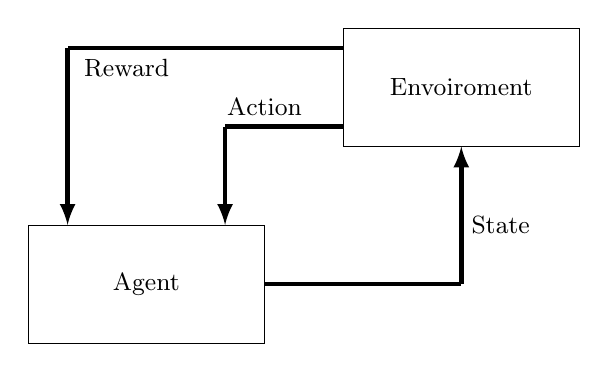
\begin{tikzpicture}[>=latex]
 %\draw [help lines] (0,0) grid [step=0.5] (8,4);
 \draw (0.5,0) rectangle ++(3cm, 1.5cm);
 \draw (4.5,2.5) rectangle ++(3cm,1.5cm);
 %\node [draw] (1.5,2) {Agent};
 \coordinate [label={[font=\small]center:Agent}] (A) at (2,0.75);
 \coordinate [label={[font=\small]center:Envoiroment}] (E) at (6,3.25);
 \draw [-, ultra thick] (3.5,0.75) -- (6,0.75);
 \draw [->, ultra thick] (6,.75) -- (6,2.5);
 \coordinate [label={[font=\small]center:State}] (S) at (6.5,1.5);
 %
 \draw [-, ultra thick] (4.5,2.75) -- (3,2.75);
 \draw [->, ultra thick] (3,2.75) -- (3,1.5);
 \coordinate [label={[font=\small]center:Action}] (T) at (3.5,3);
 %
 \draw [-, ultra thick] (4.5,3.75) -- (1,3.75);
 \draw [->, ultra thick] (1,3.75) -- (1,1.5);
 \coordinate [label={[font=\small]center:Reward}] (R) at (1.75,3.5);
\end{tikzpicture} 
\caption{reinforcement learning scheme} 
\label{fig:reinforcement-learning-scheme}
\end{figure}
%
\subsection{Unsupervised learning}
\label{subsec:unsupervised-learning}
In supervised learning, we know in advance the correct answer when we describe
our model, while in reinforcement learning we define a measure, or reward, for
the specific actions performed by the agent. In unsupervised learning, on the
other hand, we are dealing with unlabelled data or data from the unknown
structure. Using unsupervised learning techniques, we are able to observe the
structure of our data, to extract meaningful information from them without being
able to rely on the guide nor a variable known relative result, nor a reward
function. Clustering is an exploratory technique of data analysis that allows us
to organize a series of information within meaningful groups (\emph{cluster})
without having any previous knowledge of memberships in such groups. Each
cluster that can be derived during the analysis defines a group of objects that
share a certain degree of similarity, but which are more dissimilar than the
objects present in the other clusters, which is why clustering is sometimes
called \emph{``unsupervised classification"}. Clustering is an excellent
technique for structuring information to identify meaningful relationships in
the data.\cite{raschka2016machine}
%
\begin{figure}[!h]
\centering
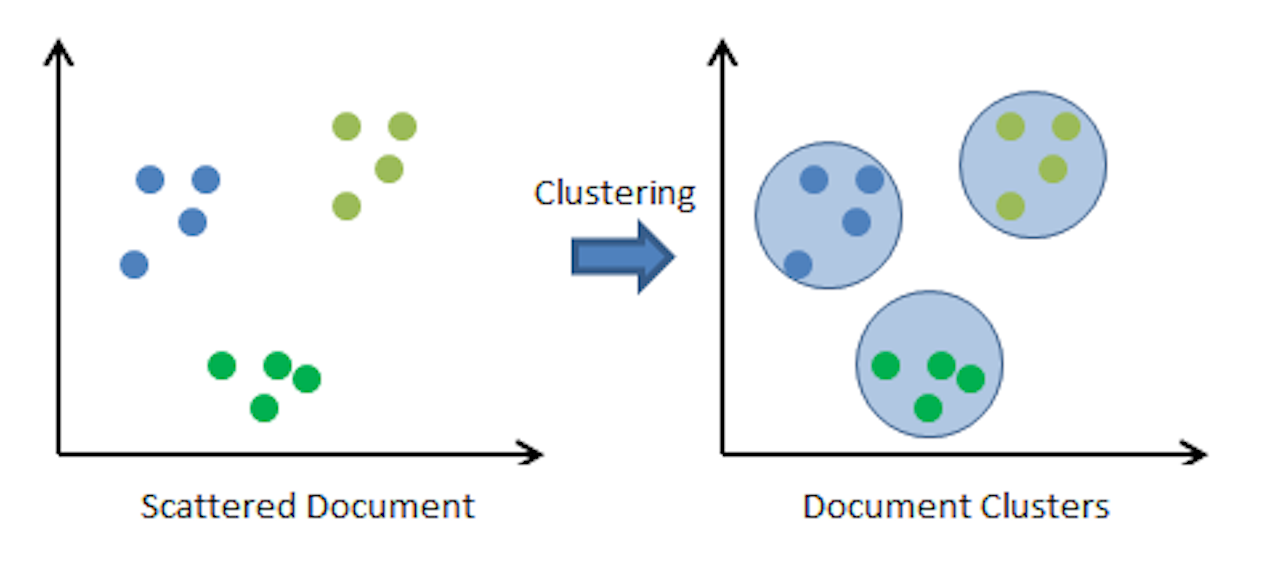
\includegraphics[width=0.70\textwidth]{cluster}
\caption{example of clustering}
\label{fig:unsupervised-learning-scheme}
\end{figure}
